\begin{example}
    \begin{figure}
        \centering
        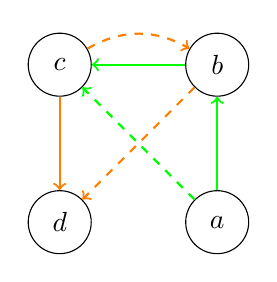
\begin{tikzpicture}[node distance={20mm},main/.style = {draw, circle,minimum size=8mm}]
            \node[main] (a)  {$a$};
            \node[main] (b) [above of=a]  {$b$};
            \node[main] (c) [left of=b] {$c$};
            \node[main] (d)  [below of=c] {$d$};
            \draw [->,green,thick] (a) -- (b);
            \draw [->,green,thick] (b) -- (c);
            \draw [->,orange,thick] (c) -- (d);
            \draw [->,green,thick,dashed] (a) -- (c);
            \draw [->,orange,thick,dashed] (c) edge[bend left] (b);
            \draw [->,orange,thick,dashed] (b) -- (d);
        \end{tikzpicture}
        \caption{ }
        \label{fig:loop}
    \end{figure}
    Loop-freedom property requires the network to not contain loop
    at any given moment \cite{network-abstractions}.
    For example consider the network in figure \ref{fig:loop}.
    Initially, there exists a path from $a$ to $d$.
    Assume that we wish to update this route to make it first visit
    $c$.
    Again, here we assume two updates replacing green and orange solid
    paths with dashed ones.
    We can encode this network using the following DyNetKAT terms:
    \begin{equation*}
        \begin{aligned}
            P           & = p!1                                             \\
            Q           & = q!1                                             \\
            N           & = F \oplus p?1;N_p \oplus q?1;N_q                 \\
            N_p         & = F_p \oplus q?1;F                                \\
            N_q         & = F_q \oplus p?1;F                                \\
            SDN         & = \delta_{\mathcal{L}}(N \parallel P \parallel Q) \\
            \mathcal{L} & = \s{p!1,p?1,q!1,q?1}
        \end{aligned}
        \qquad \qquad
        \begin{aligned}
            F    = & a\ra b \oplus a\ra c \oplus a\ra d               \\
                   & \oplus b\ra c \oplus b\ra d \oplus c\ra d        \\
            F_p  = & a\ra c \oplus a\ra d \oplus c\ra d               \\
            F_q  = & a\ra b \oplus a\ra c \oplus a\ra d               \\
                   & \oplus b\ra c \oplus b\ra b \oplus b\ra d        \\
                   & \oplus        c\ra b \oplus c\ra c \oplus c\ra d
        \end{aligned}
    \end{equation*}
    Here we assume two concurrent processes for $P$ and $Q$ for 
    updating the green and orange paths respectively.
    It is obvious that if $rcfg(q,1)$ happens while $rcfg(p,1)$ 
    has not happened yet, then a loop including $b$ and $c$ 
    would be created.
    Let $\mr{E} = \sem{SDN}$ and $\mc{M}$ be the causal model 
    of $\mr{E}$.
    Here we can assume that forwarding rules of the form $x \ra x$
    indicate the existence of a loop in the network.
    So, we can define unsafe behavior in the event structure
    as the existence of a configuration that includes an event with 
    label of the form $\alpha\cdot\pi$ where $\alpha(sw) = \pi(sw)$:
    \begin{align*}
        \f{PV} = \exists c \in \mc{F}(ES(\vec v)).
        l(c) = \alpha\cdot\pi \Rightarrow \alpha(sw) = \pi(sw)
    \end{align*}
    We can see that in $SDN$ there are only two such actions:
    $b\ra b$ and $c\ra c$.
    Like the previous example, there are two orders of execution for
    $rcfg(p,1)$ and $rcfg(q,1)$ thus we need two events to represent
    them.
    So, let's consider events $p_1$ and $p_2$ with label $rcfg(p,1)$
    and events $q_1$ and $q_2$ with label $rcfg(q,1)$.
    We also consider events $bb$ and $cc$ with labels
    $b \ra b$ and $c\ra c$ respectively.
    Figure \ref{fig:loop:es} shows a part of the $\mr{E}$ where
    events $bb$ and $cc$ are reachable.
    In this model we can introduce $M(\s{p_2},q_2) = \F$ as a cause
    of loop considering $(\e,\e,\T)$ as a witness.
    In the $\mc{M}$ functions of $M_{\e,q_2}$ and $EN_{\e,q_2}$ are
    defined as follows:
    \begin{align*}
        \f{M_{\e,q_2}}  & = Min(\e,q_2) \wedge Con(\e) \\
                        & = Min(\e,q_2)                \\
                        & =  \bigwedge_{q_2 \notin s'}
        \neg M_{s',q_2}                                \\
        \f{EN_{\e,q_2}} & = M_{\e,q_2}
    \end{align*}
    Regarding the definition of these functions if we set $M_{\s{p_2},q_2}$
    to $\T$ then $M_{\e,q_2}$ and subsequently $EN_{\e,q_2}$ becomes $\F$.
    More formally we can say:
    \begin{equation*}
        M \vDash [M_{\s{p_2},q_2} \la \T] M_{\e,q_2} = \F \wedge
        EN_{\e,q_2} = \F
    \end{equation*}
    Thus in $ES(\vec v)$ under this setting, $\s{q_2}$ and all other 
    configurations in the right branch of the 
    figure \ref{fig:loop:es} are no longer a configuration of 
    $ES(\vec v)$ which means that the property is no longer violated.
    Since we have considered and empty $\vec W$ in the witness and
    the AC2.a condition is satisfied we can conclude that 
    $M_{\s{p_2},q_2}$ is a cause of a loop in this network.
    Intuitively $M_{\s{p_2},q_2} = \F$ means $p_2$ not happening
    before $q_2$ is an actual cause of the loop.
    \begin{figure}
        \centering
        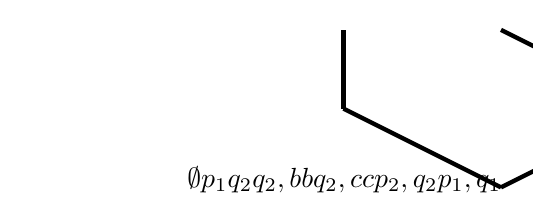
\begin{tikzpicture}
            \crd{0}{0}{$\emptyset$}
            \crd[below]{-2}{1}{$\s{p_1}$}
            \crd[below]{2}{1}{$\s{q_2}$}
            \crd[above]{2}{2}{$\s{q_2,bb}$}
            \crd[above]{4}{2}{$\s{q_2,cc}$}
            \crd[above]{0}{2}{$\s{p_2,q_2}$}
            \crd[left]{-2}{2}{$\s{p_1,q_1}$}
            \draw [ultra thick] (0,0) -- (2,1);
            \draw [ultra thick] (0,0) -- (-2,1);
            \draw [ultra thick] (2,1) -- (0,2);
            \draw [ultra thick] (2,1) -- (2,2);
            \draw [ultra thick] (2,1) -- (4,2);
            \draw [ultra thick] (-2,1) -- (-2,2);
        \end{tikzpicture}
        \caption{}
        \label{fig:loop:es}
    \end{figure}

\end{example}